\appendix

\chapter{Dica para figuras em MATLAB}

\section{Script}

\small
\lstinputlisting[language=Matlab]{./scripts/exemplos_plot.m}


\section{Figuras}

\begin{figure}[H]
    \centering
    \caption{Exemplo - extensão pdf}
    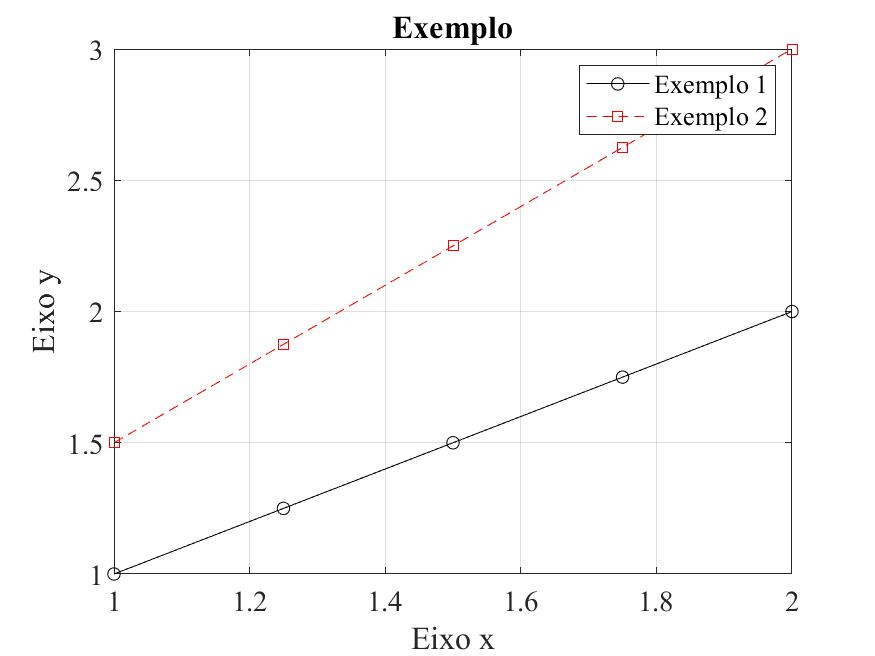
\includegraphics[trim={3.0cm 8.0cm 3.0cm 8.0cm}, clip,width=0.7\textwidth]{images/exemplo1.pdf}
\end{figure}


\begin{figure}[H]
    \centering
    \caption{Exemplo - extensão pdf}
    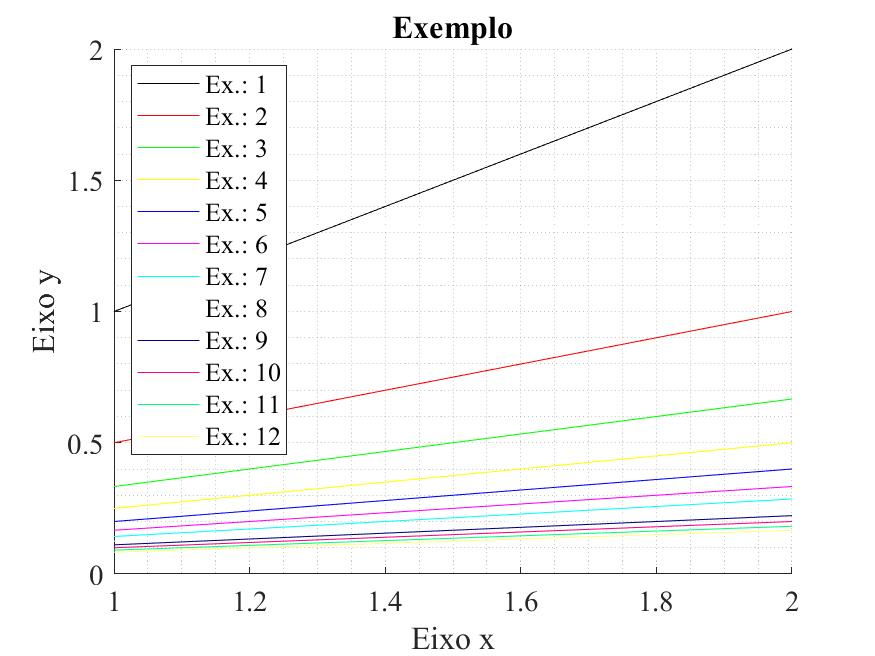
\includegraphics[trim={3.0cm 8.0cm 3.0cm 8.0cm}, clip,width=0.7\textwidth]{images/exemplo2.pdf}
\end{figure}

\begin{figure}[H]
    \centering
    \caption{Exemplo - extensão jpg}
    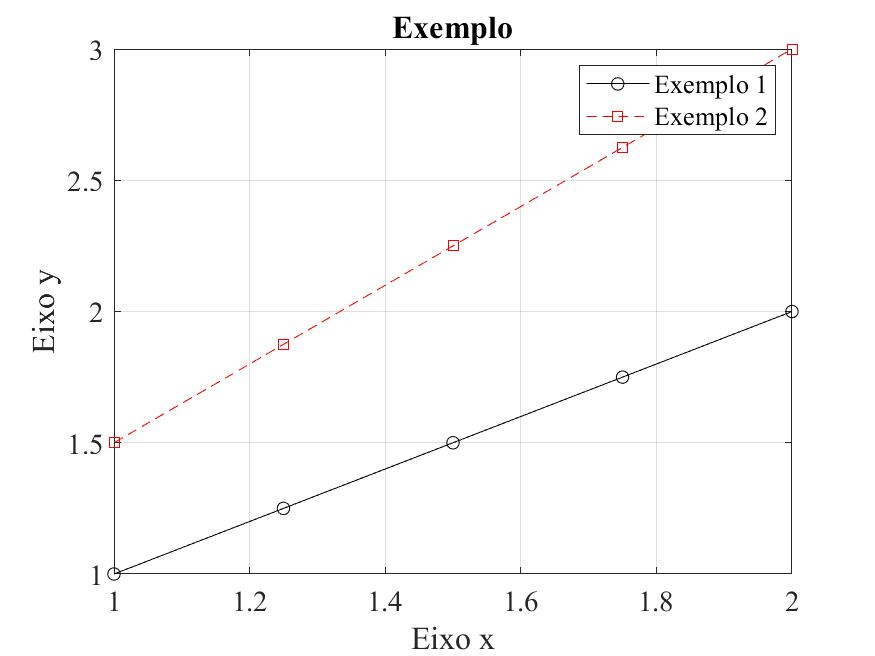
\includegraphics[width=0.7\textwidth]{images/exemplo1.jpg}
\end{figure}

\begin{figure}[H]
    \centering
    \caption{Exemplo - extensão jpg}
    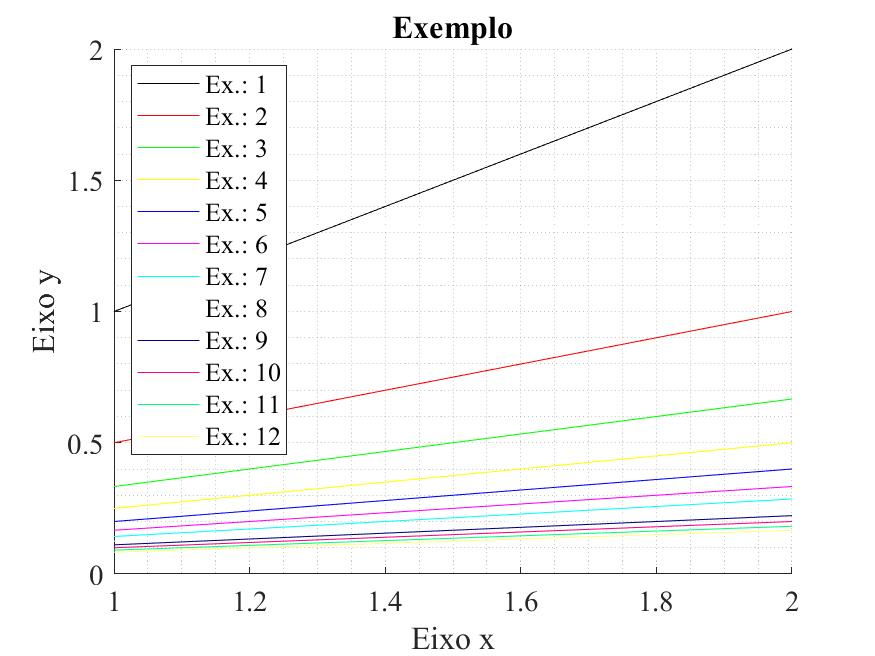
\includegraphics[width=0.7\textwidth]{images/exemplo2.jpg}
\end{figure}
